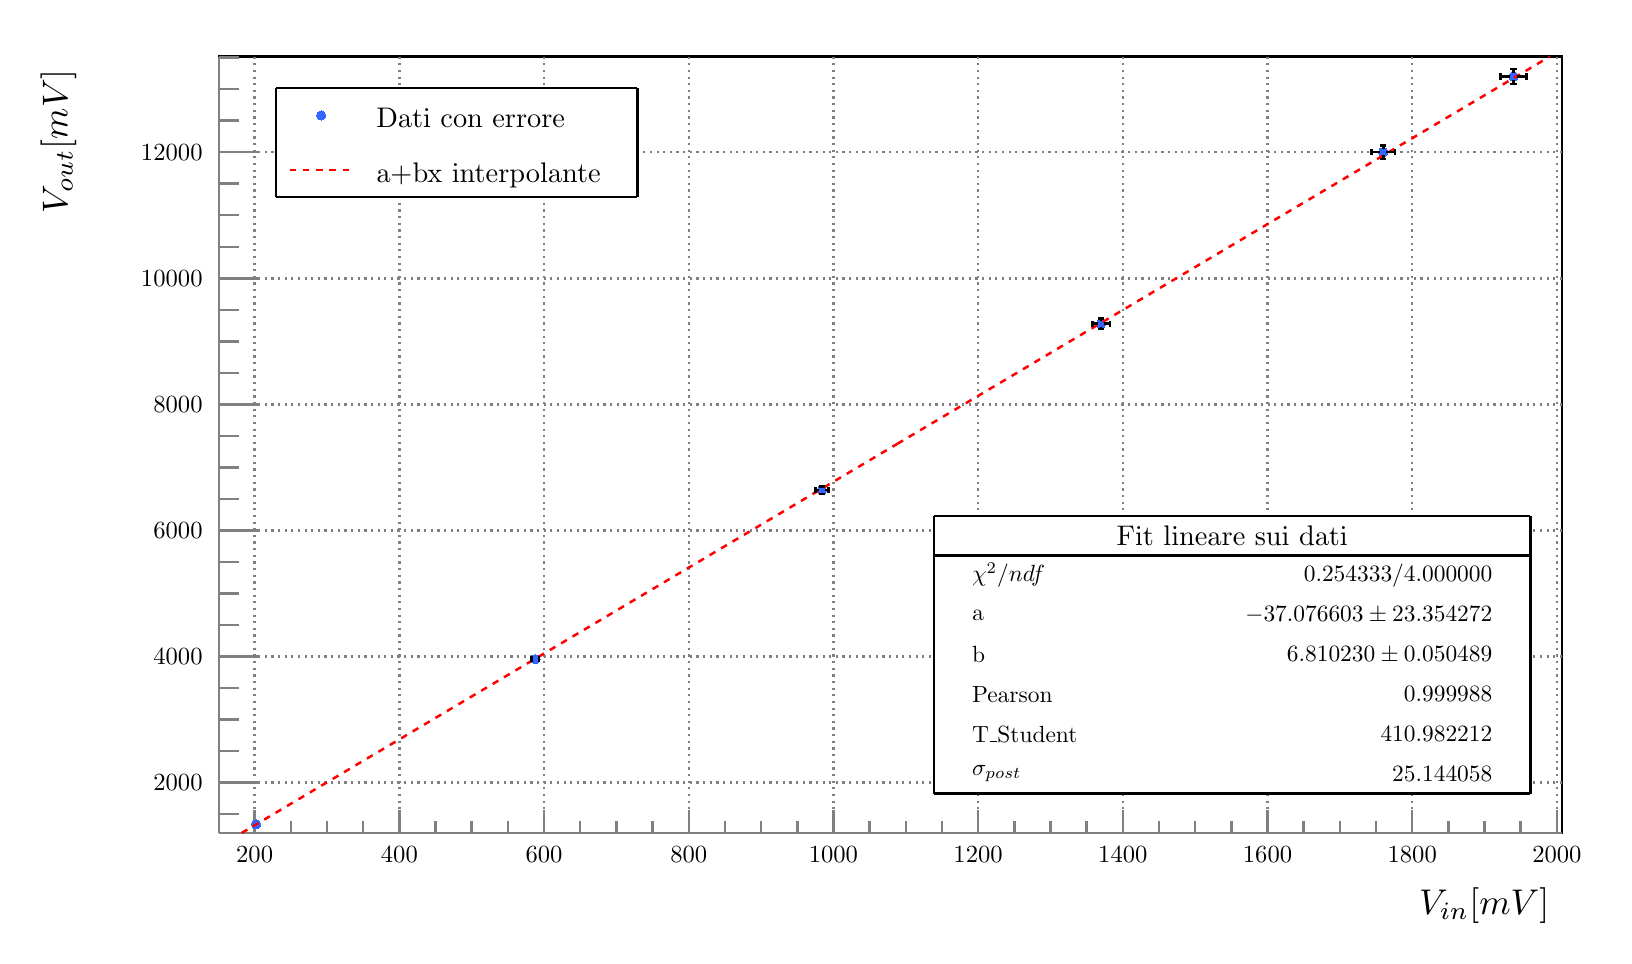
\begin{tikzpicture}
\pgfdeclareplotmark{cross} {
\pgfpathmoveto{\pgfpoint{-0.3\pgfplotmarksize}{\pgfplotmarksize}}
\pgfpathlineto{\pgfpoint{+0.3\pgfplotmarksize}{\pgfplotmarksize}}
\pgfpathlineto{\pgfpoint{+0.3\pgfplotmarksize}{0.3\pgfplotmarksize}}
\pgfpathlineto{\pgfpoint{+1\pgfplotmarksize}{0.3\pgfplotmarksize}}
\pgfpathlineto{\pgfpoint{+1\pgfplotmarksize}{-0.3\pgfplotmarksize}}
\pgfpathlineto{\pgfpoint{+0.3\pgfplotmarksize}{-0.3\pgfplotmarksize}}
\pgfpathlineto{\pgfpoint{+0.3\pgfplotmarksize}{-1.\pgfplotmarksize}}
\pgfpathlineto{\pgfpoint{-0.3\pgfplotmarksize}{-1.\pgfplotmarksize}}
\pgfpathlineto{\pgfpoint{-0.3\pgfplotmarksize}{-0.3\pgfplotmarksize}}
\pgfpathlineto{\pgfpoint{-1.\pgfplotmarksize}{-0.3\pgfplotmarksize}}
\pgfpathlineto{\pgfpoint{-1.\pgfplotmarksize}{0.3\pgfplotmarksize}}
\pgfpathlineto{\pgfpoint{-0.3\pgfplotmarksize}{0.3\pgfplotmarksize}}
\pgfpathclose
\pgfusepathqstroke
}
\pgfdeclareplotmark{cross*} {
\pgfpathmoveto{\pgfpoint{-0.3\pgfplotmarksize}{\pgfplotmarksize}}
\pgfpathlineto{\pgfpoint{+0.3\pgfplotmarksize}{\pgfplotmarksize}}
\pgfpathlineto{\pgfpoint{+0.3\pgfplotmarksize}{0.3\pgfplotmarksize}}
\pgfpathlineto{\pgfpoint{+1\pgfplotmarksize}{0.3\pgfplotmarksize}}
\pgfpathlineto{\pgfpoint{+1\pgfplotmarksize}{-0.3\pgfplotmarksize}}
\pgfpathlineto{\pgfpoint{+0.3\pgfplotmarksize}{-0.3\pgfplotmarksize}}
\pgfpathlineto{\pgfpoint{+0.3\pgfplotmarksize}{-1.\pgfplotmarksize}}
\pgfpathlineto{\pgfpoint{-0.3\pgfplotmarksize}{-1.\pgfplotmarksize}}
\pgfpathlineto{\pgfpoint{-0.3\pgfplotmarksize}{-0.3\pgfplotmarksize}}
\pgfpathlineto{\pgfpoint{-1.\pgfplotmarksize}{-0.3\pgfplotmarksize}}
\pgfpathlineto{\pgfpoint{-1.\pgfplotmarksize}{0.3\pgfplotmarksize}}
\pgfpathlineto{\pgfpoint{-0.3\pgfplotmarksize}{0.3\pgfplotmarksize}}
\pgfpathclose
\pgfusepathqfillstroke
}
\pgfdeclareplotmark{newstar} {
\pgfpathmoveto{\pgfqpoint{0pt}{\pgfplotmarksize}}
\pgfpathlineto{\pgfqpointpolar{44}{0.5\pgfplotmarksize}}
\pgfpathlineto{\pgfqpointpolar{18}{\pgfplotmarksize}}
\pgfpathlineto{\pgfqpointpolar{-20}{0.5\pgfplotmarksize}}
\pgfpathlineto{\pgfqpointpolar{-54}{\pgfplotmarksize}}
\pgfpathlineto{\pgfqpointpolar{-90}{0.5\pgfplotmarksize}}
\pgfpathlineto{\pgfqpointpolar{234}{\pgfplotmarksize}}
\pgfpathlineto{\pgfqpointpolar{198}{0.5\pgfplotmarksize}}
\pgfpathlineto{\pgfqpointpolar{162}{\pgfplotmarksize}}
\pgfpathlineto{\pgfqpointpolar{134}{0.5\pgfplotmarksize}}
\pgfpathclose
\pgfusepathqstroke
}
\pgfdeclareplotmark{newstar*} {
\pgfpathmoveto{\pgfqpoint{0pt}{\pgfplotmarksize}}
\pgfpathlineto{\pgfqpointpolar{44}{0.5\pgfplotmarksize}}
\pgfpathlineto{\pgfqpointpolar{18}{\pgfplotmarksize}}
\pgfpathlineto{\pgfqpointpolar{-20}{0.5\pgfplotmarksize}}
\pgfpathlineto{\pgfqpointpolar{-54}{\pgfplotmarksize}}
\pgfpathlineto{\pgfqpointpolar{-90}{0.5\pgfplotmarksize}}
\pgfpathlineto{\pgfqpointpolar{234}{\pgfplotmarksize}}
\pgfpathlineto{\pgfqpointpolar{198}{0.5\pgfplotmarksize}}
\pgfpathlineto{\pgfqpointpolar{162}{\pgfplotmarksize}}
\pgfpathlineto{\pgfqpointpolar{134}{0.5\pgfplotmarksize}}
\pgfpathclose
\pgfusepathqfillstroke
}
\definecolor{c}{rgb}{1,1,1};
\draw [color=c, fill=c] (0,0) rectangle (20,11.523);
\draw [color=c, fill=c] (2.42485,1.30261) rectangle (19.479,11.1623);
\definecolor{c}{rgb}{0,0,0};
\draw [c,line width=0.9] (2.42485,1.30261) -- (2.42485,11.1623) -- (19.479,11.1623) -- (19.479,1.30261) -- (2.42485,1.30261);
\definecolor{c}{rgb}{1,1,1};
\draw [color=c, fill=c] (2.42485,1.30261) rectangle (19.479,11.1623);
\definecolor{c}{rgb}{0,0,0};
\draw [c,line width=0.9] (2.42485,1.30261) -- (2.42485,11.1623) -- (19.479,11.1623) -- (19.479,1.30261) -- (2.42485,1.30261);
\definecolor{c}{rgb}{0.5,0.5,0.5};
\draw [c,line width=0.9] (2.42485,1.30261) -- (19.479,1.30261);
\draw [c,dash pattern=on 0.80pt off 1.60pt ,line width=0.9] (2.87566,11.1623) -- (2.87566,1.30261);
\draw [c,dash pattern=on 0.80pt off 1.60pt ,line width=0.9] (4.71327,11.1623) -- (4.71327,1.30261);
\draw [c,dash pattern=on 0.80pt off 1.60pt ,line width=0.9] (6.55087,11.1623) -- (6.55087,1.30261);
\draw [c,dash pattern=on 0.80pt off 1.60pt ,line width=0.9] (8.38848,11.1623) -- (8.38848,1.30261);
\draw [c,dash pattern=on 0.80pt off 1.60pt ,line width=0.9] (10.2261,11.1623) -- (10.2261,1.30261);
\draw [c,dash pattern=on 0.80pt off 1.60pt ,line width=0.9] (12.0637,11.1623) -- (12.0637,1.30261);
\draw [c,dash pattern=on 0.80pt off 1.60pt ,line width=0.9] (13.9013,11.1623) -- (13.9013,1.30261);
\draw [c,dash pattern=on 0.80pt off 1.60pt ,line width=0.9] (15.7389,11.1623) -- (15.7389,1.30261);
\draw [c,dash pattern=on 0.80pt off 1.60pt ,line width=0.9] (17.5765,11.1623) -- (17.5765,1.30261);
\draw [c,dash pattern=on 0.80pt off 1.60pt ,line width=0.9] (19.4141,11.1623) -- (19.4141,1.30261);
\draw [c,dash pattern=on 0.80pt off 1.60pt ,line width=0.9] (2.87566,11.1623) -- (2.87566,1.30261);
\draw [c,dash pattern=on 0.80pt off 1.60pt ,line width=0.9] (19.4141,11.1623) -- (19.4141,1.30261);
\draw [c,line width=0.9] (2.42485,1.30261) -- (2.42485,11.1623);
\draw [c,dash pattern=on 0.80pt off 1.60pt ,line width=0.9] (19.479,1.94115) -- (2.42485,1.94115);
\draw [c,dash pattern=on 0.80pt off 1.60pt ,line width=0.9] (19.479,3.54263) -- (2.42485,3.54263);
\draw [c,dash pattern=on 0.80pt off 1.60pt ,line width=0.9] (19.479,5.14411) -- (2.42485,5.14411);
\draw [c,dash pattern=on 0.80pt off 1.60pt ,line width=0.9] (19.479,6.74559) -- (2.42485,6.74559);
\draw [c,dash pattern=on 0.80pt off 1.60pt ,line width=0.9] (19.479,8.34707) -- (2.42485,8.34707);
\draw [c,dash pattern=on 0.80pt off 1.60pt ,line width=0.9] (19.479,9.94855) -- (2.42485,9.94855);
\draw [c,dash pattern=on 0.80pt off 1.60pt ,line width=0.9] (19.479,1.94115) -- (2.42485,1.94115);
\draw [c,dash pattern=on 0.80pt off 1.60pt ,line width=0.9] (19.479,9.94855) -- (2.42485,9.94855);
\draw [c,line width=0.9] (2.42485,1.30261) -- (19.479,1.30261);
\draw [c,line width=0.9] (2.87566,1.59738) -- (2.87566,1.30261);
\draw [c,line width=0.9] (3.33506,1.44999) -- (3.33506,1.30261);
\draw [c,line width=0.9] (3.79446,1.44999) -- (3.79446,1.30261);
\draw [c,line width=0.9] (4.25386,1.44999) -- (4.25386,1.30261);
\draw [c,line width=0.9] (4.71327,1.59738) -- (4.71327,1.30261);
\draw [c,line width=0.9] (5.17267,1.44999) -- (5.17267,1.30261);
\draw [c,line width=0.9] (5.63207,1.44999) -- (5.63207,1.30261);
\draw [c,line width=0.9] (6.09147,1.44999) -- (6.09147,1.30261);
\draw [c,line width=0.9] (6.55087,1.59738) -- (6.55087,1.30261);
\draw [c,line width=0.9] (7.01028,1.44999) -- (7.01028,1.30261);
\draw [c,line width=0.9] (7.46968,1.44999) -- (7.46968,1.30261);
\draw [c,line width=0.9] (7.92908,1.44999) -- (7.92908,1.30261);
\draw [c,line width=0.9] (8.38848,1.59738) -- (8.38848,1.30261);
\draw [c,line width=0.9] (8.84789,1.44999) -- (8.84789,1.30261);
\draw [c,line width=0.9] (9.30729,1.44999) -- (9.30729,1.30261);
\draw [c,line width=0.9] (9.76669,1.44999) -- (9.76669,1.30261);
\draw [c,line width=0.9] (10.2261,1.59738) -- (10.2261,1.30261);
\draw [c,line width=0.9] (10.6855,1.44999) -- (10.6855,1.30261);
\draw [c,line width=0.9] (11.1449,1.44999) -- (11.1449,1.30261);
\draw [c,line width=0.9] (11.6043,1.44999) -- (11.6043,1.30261);
\draw [c,line width=0.9] (12.0637,1.59738) -- (12.0637,1.30261);
\draw [c,line width=0.9] (12.5231,1.44999) -- (12.5231,1.30261);
\draw [c,line width=0.9] (12.9825,1.44999) -- (12.9825,1.30261);
\draw [c,line width=0.9] (13.4419,1.44999) -- (13.4419,1.30261);
\draw [c,line width=0.9] (13.9013,1.59738) -- (13.9013,1.30261);
\draw [c,line width=0.9] (14.3607,1.44999) -- (14.3607,1.30261);
\draw [c,line width=0.9] (14.8201,1.44999) -- (14.8201,1.30261);
\draw [c,line width=0.9] (15.2795,1.44999) -- (15.2795,1.30261);
\draw [c,line width=0.9] (15.7389,1.59738) -- (15.7389,1.30261);
\draw [c,line width=0.9] (16.1983,1.44999) -- (16.1983,1.30261);
\draw [c,line width=0.9] (16.6577,1.44999) -- (16.6577,1.30261);
\draw [c,line width=0.9] (17.1171,1.44999) -- (17.1171,1.30261);
\draw [c,line width=0.9] (17.5765,1.59738) -- (17.5765,1.30261);
\draw [c,line width=0.9] (18.0359,1.44999) -- (18.0359,1.30261);
\draw [c,line width=0.9] (18.4953,1.44999) -- (18.4953,1.30261);
\draw [c,line width=0.9] (18.9547,1.44999) -- (18.9547,1.30261);
\draw [c,line width=0.9] (19.4141,1.59738) -- (19.4141,1.30261);
\draw [c,line width=0.9] (2.87566,1.59738) -- (2.87566,1.30261);
\draw [c,line width=0.9] (19.4141,1.59738) -- (19.4141,1.30261);
\definecolor{c}{rgb}{0,0,0};
\draw [anchor=base] (2.87566,0.922345) node[scale=0.890168, color=c, rotate=0]{200};
\draw [anchor=base] (4.71327,0.922345) node[scale=0.890168, color=c, rotate=0]{400};
\draw [anchor=base] (6.55087,0.922345) node[scale=0.890168, color=c, rotate=0]{600};
\draw [anchor=base] (8.38848,0.922345) node[scale=0.890168, color=c, rotate=0]{800};
\draw [anchor=base] (10.2261,0.922345) node[scale=0.890168, color=c, rotate=0]{1000};
\draw [anchor=base] (12.0637,0.922345) node[scale=0.890168, color=c, rotate=0]{1200};
\draw [anchor=base] (13.9013,0.922345) node[scale=0.890168, color=c, rotate=0]{1400};
\draw [anchor=base] (15.7389,0.922345) node[scale=0.890168, color=c, rotate=0]{1600};
\draw [anchor=base] (17.5765,0.922345) node[scale=0.890168, color=c, rotate=0]{1800};
\draw [anchor=base] (19.4141,0.922345) node[scale=0.890168, color=c, rotate=0]{2000};
\draw [anchor= east] (19.479,0.380762) node[scale=1.29074, color=c, rotate=0]{$V_{in} [mV]$};
\definecolor{c}{rgb}{0.5,0.5,0.5};
\draw [c,line width=0.9] (2.42485,1.30261) -- (2.42485,11.1623);
\draw [c,line width=0.9] (2.93824,1.94115) -- (2.42485,1.94115);
\draw [c,line width=0.9] (2.68155,2.34152) -- (2.42485,2.34152);
\draw [c,line width=0.9] (2.68155,2.74189) -- (2.42485,2.74189);
\draw [c,line width=0.9] (2.68155,3.14226) -- (2.42485,3.14226);
\draw [c,line width=0.9] (2.93824,3.54263) -- (2.42485,3.54263);
\draw [c,line width=0.9] (2.68155,3.943) -- (2.42485,3.943);
\draw [c,line width=0.9] (2.68155,4.34337) -- (2.42485,4.34337);
\draw [c,line width=0.9] (2.68155,4.74374) -- (2.42485,4.74374);
\draw [c,line width=0.9] (2.93824,5.14411) -- (2.42485,5.14411);
\draw [c,line width=0.9] (2.68155,5.54448) -- (2.42485,5.54448);
\draw [c,line width=0.9] (2.68155,5.94485) -- (2.42485,5.94485);
\draw [c,line width=0.9] (2.68155,6.34522) -- (2.42485,6.34522);
\draw [c,line width=0.9] (2.93824,6.74559) -- (2.42485,6.74559);
\draw [c,line width=0.9] (2.68155,7.14596) -- (2.42485,7.14596);
\draw [c,line width=0.9] (2.68155,7.54633) -- (2.42485,7.54633);
\draw [c,line width=0.9] (2.68155,7.9467) -- (2.42485,7.9467);
\draw [c,line width=0.9] (2.93824,8.34707) -- (2.42485,8.34707);
\draw [c,line width=0.9] (2.68155,8.74744) -- (2.42485,8.74744);
\draw [c,line width=0.9] (2.68155,9.14781) -- (2.42485,9.14781);
\draw [c,line width=0.9] (2.68155,9.54818) -- (2.42485,9.54818);
\draw [c,line width=0.9] (2.93824,9.94855) -- (2.42485,9.94855);
\draw [c,line width=0.9] (2.93824,1.94115) -- (2.42485,1.94115);
\draw [c,line width=0.9] (2.68155,1.54078) -- (2.42485,1.54078);
\draw [c,line width=0.9] (2.93824,9.94855) -- (2.42485,9.94855);
\draw [c,line width=0.9] (2.68155,10.3489) -- (2.42485,10.3489);
\draw [c,line width=0.9] (2.68155,10.7493) -- (2.42485,10.7493);
\draw [c,line width=0.9] (2.68155,11.1497) -- (2.42485,11.1497);
\definecolor{c}{rgb}{0,0,0};
\draw [anchor= east] (2.32485,1.94115) node[scale=0.890168, color=c, rotate=0]{2000};
\draw [anchor= east] (2.32485,3.54263) node[scale=0.890168, color=c, rotate=0]{4000};
\draw [anchor= east] (2.32485,5.14411) node[scale=0.890168, color=c, rotate=0]{6000};
\draw [anchor= east] (2.32485,6.74559) node[scale=0.890168, color=c, rotate=0]{8000};
\draw [anchor= east] (2.32485,8.34707) node[scale=0.890168, color=c, rotate=0]{10000};
\draw [anchor= east] (2.32485,9.94855) node[scale=0.890168, color=c, rotate=0]{12000};
\draw [anchor= east] (0.382766,11.1623) node[scale=1.29074, color=c, rotate=90]{$V_{out} [mV]$};
\definecolor{c}{rgb}{0.2,0.4,1};
\foreach \P in {(2.89403,1.41266), (6.44062,3.5106), (10.0791,5.65658), (13.6257,7.77054), (17.209,9.94855), (18.8629,10.9094)}{\draw[mark options={color=c,fill=c},mark size=1.681682pt, line width=0.000000pt, mark=*] plot coordinates {\P};}
\definecolor{c}{rgb}{1,0,0};
\draw [c,dash pattern=on 2.40pt off 2.40pt ,line width=0.9] (2.71051,1.30261) -- (2.8512,1.38611);
\draw [c,dash pattern=on 2.40pt off 2.40pt ,line width=0.9] (2.8512,1.38611) -- (3.02174,1.48733) -- (3.19228,1.58855) -- (3.36283,1.68976) -- (3.53337,1.79098) -- (3.70391,1.8922) -- (3.87445,1.99342) -- (4.04499,2.09464) -- (4.21553,2.19586) --
 (4.38607,2.29708) -- (4.55661,2.39829) -- (4.72715,2.49951) -- (4.8977,2.60073) -- (5.06824,2.70195) -- (5.23878,2.80317) -- (5.40932,2.90439) -- (5.57986,3.0056) -- (5.7504,3.10682) -- (5.92094,3.20804) -- (6.09148,3.30926) -- (6.26202,3.41048) --
 (6.43257,3.5117) -- (6.60311,3.61291) -- (6.77365,3.71413) -- (6.94419,3.81535) -- (7.11473,3.91657) -- (7.28527,4.01779) -- (7.45581,4.11901) -- (7.62635,4.22023) -- (7.79689,4.32144) -- (7.96743,4.42266) -- (8.13798,4.52388) -- (8.30852,4.6251) --
 (8.47906,4.72632) -- (8.6496,4.82754) -- (8.82014,4.92875) -- (8.99068,5.02997) -- (9.16122,5.13119) -- (9.33176,5.23241) -- (9.50231,5.33363) -- (9.67285,5.43485) -- (9.84339,5.53607) -- (10.0139,5.63728) -- (10.1845,5.7385) -- (10.355,5.83972) --
 (10.5256,5.94094) -- (10.6961,6.04216) -- (10.8666,6.14338) -- (11.0372,6.24459);
\draw [c,dash pattern=on 2.40pt off 2.40pt ,line width=0.9] (11.0372,6.24459) -- (11.2077,6.34581) -- (11.3783,6.44703) -- (11.5488,6.54825) -- (11.7193,6.64947) -- (11.8899,6.75069) -- (12.0604,6.85191) -- (12.231,6.95312) -- (12.4015,7.05434) --
 (12.572,7.15556) -- (12.7426,7.25678) -- (12.9131,7.358) -- (13.0837,7.45922) -- (13.2542,7.56043) -- (13.4247,7.66165) -- (13.5953,7.76287) -- (13.7658,7.86409) -- (13.9364,7.96531) -- (14.1069,8.06653) -- (14.2775,8.16775) -- (14.448,8.26896) --
 (14.6185,8.37018) -- (14.7891,8.4714) -- (14.9596,8.57262) -- (15.1302,8.67384) -- (15.3007,8.77506) -- (15.4712,8.87627) -- (15.6418,8.97749) -- (15.8123,9.07871) -- (15.9829,9.17993) -- (16.1534,9.28115) -- (16.3239,9.38237) -- (16.4945,9.48359)
 -- (16.665,9.5848) -- (16.8356,9.68602) -- (17.0061,9.78724) -- (17.1767,9.88846) -- (17.3472,9.98968) -- (17.5177,10.0909) -- (17.6883,10.1921) -- (17.8588,10.2933) -- (18.0294,10.3946) -- (18.1999,10.4958) -- (18.3704,10.597) -- (18.541,10.6982)
 -- (18.7115,10.7994) -- (18.8821,10.9006) -- (19.0526,11.0019) -- (19.2231,11.1031) -- (19.323,11.1623);
\definecolor{c}{rgb}{0,0,0};
\draw [c,line width=0.9] (6.40054,3.5106) -- (6.39255,3.5106);
\draw [c,line width=0.9] (6.39255,3.47052) -- (6.39255,3.55068);
\draw [c,line width=0.9] (6.4807,3.5106) -- (6.48869,3.5106);
\draw [c,line width=0.9] (6.48869,3.47052) -- (6.48869,3.55068);
\draw [c,line width=0.9] (10.039,5.65658) -- (9.99774,5.65658);
\draw [c,line width=0.9] (9.99774,5.6165) -- (9.99774,5.69666);
\draw [c,line width=0.9] (10.1192,5.65658) -- (10.1604,5.65658);
\draw [c,line width=0.9] (10.1604,5.6165) -- (10.1604,5.69666);
\draw [c,line width=0.9] (10.0791,5.69666) -- (10.0791,5.70362);
\draw [c,line width=0.9] (10.039,5.70362) -- (10.1192,5.70362);
\draw [c,line width=0.9] (10.0791,5.6165) -- (10.0791,5.60955);
\draw [c,line width=0.9] (10.039,5.60955) -- (10.1192,5.60955);
\draw [c,line width=0.9] (13.5856,7.77054) -- (13.5144,7.77054);
\draw [c,line width=0.9] (13.5144,7.73046) -- (13.5144,7.81062);
\draw [c,line width=0.9] (13.6657,7.77054) -- (13.7369,7.77054);
\draw [c,line width=0.9] (13.7369,7.73046) -- (13.7369,7.81062);
\draw [c,line width=0.9] (13.6257,7.81062) -- (13.6257,7.8377);
\draw [c,line width=0.9] (13.5856,7.8377) -- (13.6657,7.8377);
\draw [c,line width=0.9] (13.6257,7.73046) -- (13.6257,7.70338);
\draw [c,line width=0.9] (13.5856,7.70338) -- (13.6657,7.70338);
\draw [c,line width=0.9] (17.1689,9.94855) -- (17.0585,9.94855);
\draw [c,line width=0.9] (17.0585,9.90847) -- (17.0585,9.98864);
\draw [c,line width=0.9] (17.2491,9.94855) -- (17.3595,9.94855);
\draw [c,line width=0.9] (17.3595,9.90847) -- (17.3595,9.98864);
\draw [c,line width=0.9] (17.209,9.98864) -- (17.209,10.034);
\draw [c,line width=0.9] (17.1689,10.034) -- (17.2491,10.034);
\draw [c,line width=0.9] (17.209,9.90847) -- (17.209,9.86315);
\draw [c,line width=0.9] (17.1689,9.86315) -- (17.2491,9.86315);
\draw [c,line width=0.9] (18.8228,10.9094) -- (18.6989,10.9094);
\draw [c,line width=0.9] (18.6989,10.8694) -- (18.6989,10.9495);
\draw [c,line width=0.9] (18.9029,10.9094) -- (19.0268,10.9094);
\draw [c,line width=0.9] (19.0268,10.8694) -- (19.0268,10.9495);
\draw [c,line width=0.9] (18.8629,10.9495) -- (18.8629,11.003);
\draw [c,line width=0.9] (18.8228,11.003) -- (18.9029,11.003);
\draw [c,line width=0.9] (18.8629,10.8694) -- (18.8629,10.8159);
\draw [c,line width=0.9] (18.8228,10.8159) -- (18.9029,10.8159);
\definecolor{c}{rgb}{1,1,1};
\draw [color=c, fill=c] (3.14629,9.37876) rectangle (7.73547,10.7615);
\definecolor{c}{rgb}{0,0,0};
\draw [c,line width=0.9] (3.14629,9.37876) -- (7.73547,9.37876);
\draw [c,line width=0.9] (7.73547,9.37876) -- (7.73547,10.7615);
\draw [c,line width=0.9] (7.73547,10.7615) -- (3.14629,10.7615);
\draw [c,line width=0.9] (3.14629,10.7615) -- (3.14629,9.37876);
\draw [anchor=base west] (4.29359,10.2603) node[scale=1.02369, color=c, rotate=0]{Dati con errore};
\definecolor{c}{rgb}{0.2,0.4,1};
\foreach \P in {(3.71994,10.4158)}{\draw[mark options={color=c,fill=c},mark size=1.681682pt, line width=0.000000pt, mark=*] plot coordinates {\P};}
\definecolor{c}{rgb}{0,0,0};
\draw [anchor=base west] (4.29359,9.56889) node[scale=1.02369, color=c, rotate=0]{a+bx interpolante};
\definecolor{c}{rgb}{1,0,0};
\draw [c,dash pattern=on 2.40pt off 2.40pt ,line width=0.9] (3.31839,9.72445) -- (4.12149,9.72445);
\definecolor{c}{rgb}{1,1,1};
\draw [color=c, fill=c] (11.503,1.80361) rectangle (19.0782,5.33066);
\definecolor{c}{rgb}{0,0,0};
\draw [c,line width=0.9] (11.503,1.80361) -- (19.0782,1.80361);
\draw [c,line width=0.9] (19.0782,1.80361) -- (19.0782,5.33066);
\draw [c,line width=0.9] (19.0782,5.33066) -- (11.503,5.33066);
\draw [c,line width=0.9] (11.503,5.33066) -- (11.503,1.80361);
\draw (15.2906,5.07873) node[scale=1.02369, color=c, rotate=0]{Fit lineare sui dati};
\draw [c,line width=0.9] (11.503,4.8268) -- (19.0782,4.8268);
\draw [anchor= west] (11.8818,4.57486) node[scale=0.84566, color=c, rotate=0]{$\chi^{2} / ndf $};
\draw [anchor= east] (18.6994,4.57486) node[scale=0.84566, color=c, rotate=0]{0.254333/4.000000};
\draw [anchor= west] (11.8818,4.071) node[scale=0.84566, color=c, rotate=0]{a        };
\draw [anchor= east] (18.6994,4.071) node[scale=0.84566, color=c, rotate=0]{$ -37.076603\pm23.354272$};
\draw [anchor= west] (11.8818,3.56713) node[scale=0.84566, color=c, rotate=0]{b        };
\draw [anchor= east] (18.6994,3.56713) node[scale=0.84566, color=c, rotate=0]{$ 6.810230\pm0.050489$};
\draw [anchor= west] (11.8818,3.06327) node[scale=0.84566, color=c, rotate=0]{Pearson        };
\draw [anchor= east] (18.6994,3.06327) node[scale=0.84566, color=c, rotate=0]{ 0.999988};
\draw [anchor= west] (11.8818,2.5594) node[scale=0.84566, color=c, rotate=0]{T\_Student        };
\draw [anchor= east] (18.6994,2.5594) node[scale=0.84566, color=c, rotate=0]{ 410.982212};
\draw [anchor= west] (11.8818,2.05554) node[scale=0.84566, color=c, rotate=0]{$\sigma_{post}        $};
\draw [anchor= east] (18.6994,2.05554) node[scale=0.84566, color=c, rotate=0]{ 25.144058};
\end{tikzpicture}
